
\documentclass[11pt,a4paper]{article}
\usepackage[utf8]{inputenc}
\usepackage[T1]{fontenc}
\usepackage[french]{babel}
\usepackage[margin=2.1cm]{geometry}
\usepackage{amsmath,graphicx,booktabs,float,longtable}
\usepackage[hidelinks]{hyperref}
\graphicspath{{../resultats/}}
\hypersetup{pdfauthor={Houssam MAKHLOUK},pdftitle={TP3 - Intégration SLAM et cartographie}}
\begin{document}
\hypersetup{pageanchor=false}
\begin{titlepage}\centering
\vspace*{1cm}{\Large\bfseries EIGSI\par}
\vspace{.4cm}{\large Année universitaire 2026/2027\par}
\vspace{2cm}{\large RAPPORT DE TRAVAUX PRATIQUES\par}
\vspace{.8cm}\rule{.9\textwidth}{1pt}\par\vspace{.6cm}
{\Huge\bfseries TP -- Jour 3\par}\vspace{.6cm}
{\LARGE Intégration SLAM et cartographie de la salle\par}
\vspace{.6cm}\rule{.9\textwidth}{1pt}
\vfill{\large Réalisé par\par}\vspace{.3cm}
{\LARGE\bfseries Houssam MAKHLOUK\par}
\vspace{.4cm}{\large Étudiant à EIGSI\par}
\vfill
\end{titlepage}
\pagenumbering{roman}\hypersetup{pageanchor=true}
\tableofcontents\clearpage\pagenumbering{arabic}

\section{Objectif et continuité des TP}
Le TP1 fournit la lecture des CSV, la conversion des coordonnées, une grille
d'occupation et une carte vectorielle. Le TP2 fournit la localisation entre
scans. Ce TP3 les enchaîne : après chaque estimation de pose, le nouveau scan
est projeté dans le repère global et inséré dans les deux cartes. Le rejeu
est incrémental : le scan courant n'utilise que la carte construite avec les
scans précédents. Il s'agit d'un début de SLAM sur des scans enregistrés. La carte n'est pas corrigée par
fermeture de boucle ni par optimisation globale des poses.

\section{Données, sélection et repères}
Le lot sélectionné comprend quatre scans du TP1 et les trois tours A et B du
TP2, soit 10 scans. Ils sont annoncés à une même hauteur de 1,90 m dans
les métadonnées ou le protocole. Cette hauteur n'a pas été mesurée par le
LiDAR. Les acquisitions N1, N2, N3, N5 et N6 ont une hauteur estimée entre
1,00 et 1,20 m ; N4 a été pris au sol. Ces acquisitions restent disponibles
dans le TP2, mais ne sont pas superposées à cette coupe 2D.

Le scan 1 du TP1 fixe le repère $(0,0,0^\circ)$. Les scans sont rejoués dans
l'ordre d'acquisition. Aucune pose sauvegardée
des TP1 et TP2 n'est utilisée pour localiser les scans suivants. Les poses
initiales sont générées avec la dernière pose estimée et les centres des
nuages pour quatre orientations candidates. Les fichiers sources et leurs coordonnées locales sont
conservés ; les coordonnées globales produites sont exportées séparément.

\section{Algorithme de localisation et de cartographie}
\subsection{Boucle scan par scan}
Pour chaque scan $S_k$, l'algorithme extrait les points valides entre 0,15 et
12 m. Les impacts déjà placés forment une référence croissante. La méthode
\texttt{scan\_coarse\_icp} du TP2 cherche la pose par recherche multirésolution,
puis affine par ICP. Le nuage de référence est réduit à un représentant par
cellule de 7 cm, puis au maximum à 700 points pour limiter le temps de calcul.
Cinq hypothèses initiales sont essayées : la dernière pose et quatre rotations
relatives à celle-ci, recentrées sur le nuage déjà cartographié. La pose au
coût le plus faible est évaluée avant chaque mise à jour de carte.

Un contrôle refuse l'ajout si moins de 32\% des points sont à 30 cm de la
référence ou si le score plafonné dépasse 0,11 m$^2$. Ces seuils servent
à limiter les fusions manifestement incompatibles ; ils ne démontrent pas
qu'une pose acceptée est géométriquement exacte.

\subsection{Mise à jour des cartes}
La grid map a une résolution de 0,08 m. Elle contient trois états : inconnu
$(-1)$, libre $(0)$ et occupé $(100)$. Chaque rayon marque les cellules
traversées comme libres et la cellule d'impact comme occupée. Le calcul utilise
la pose estimée pour le scan courant. La grille s'agrandit en cellules
inconnues lorsqu'un nouvel impact sort de ses bornes. La carte vectorielle extrait des segments
du scan local, les place dans le repère global et fusionne ceux qui sont
proches en position et orientation. Le découpage par rayons libres est désactivé
ici afin que de petites erreurs de pose ne suppriment pas les anciens segments.
Une mise à jour automatique de la géométrie des poses passées n'est pas faite.

\subsection{Contrôles reproductibles}
Un test de simulation utilise 80 points déterministes et une pose connue
$(0,70\,\mathrm{m},-0,35\,\mathrm{m},25^\circ)$. Le recalage retrouve cette pose
à moins de 0,03 m sur chaque coordonnée et 0,03$^\circ$ sur l'orientation.
Un second test vérifie l'agrandissement de la grille avant l'insertion d'un
rayon nouveau. Un rejeu de deux scans réels vérifie que les cartes et les
exports sont produits sans lecture des poses sauvegardées. Ces tests ne
remplacent pas une mesure indépendante dans la salle.

\section{Partie SLAM illustrée}
La figure suivante montre un exemple du cycle localisation puis cartographie.
Le scan 3 arrive dans son repère local alors que la carte ne contient que le
scan 1 : le scan 2 a été écarté par le contrôle de qualité. Après recalage,
les murs communs du scan 3 se superposent à ceux de la carte. Les segments
verts sont un échantillon de correspondances à moins de 20 cm.
\begin{figure}[H]\centering
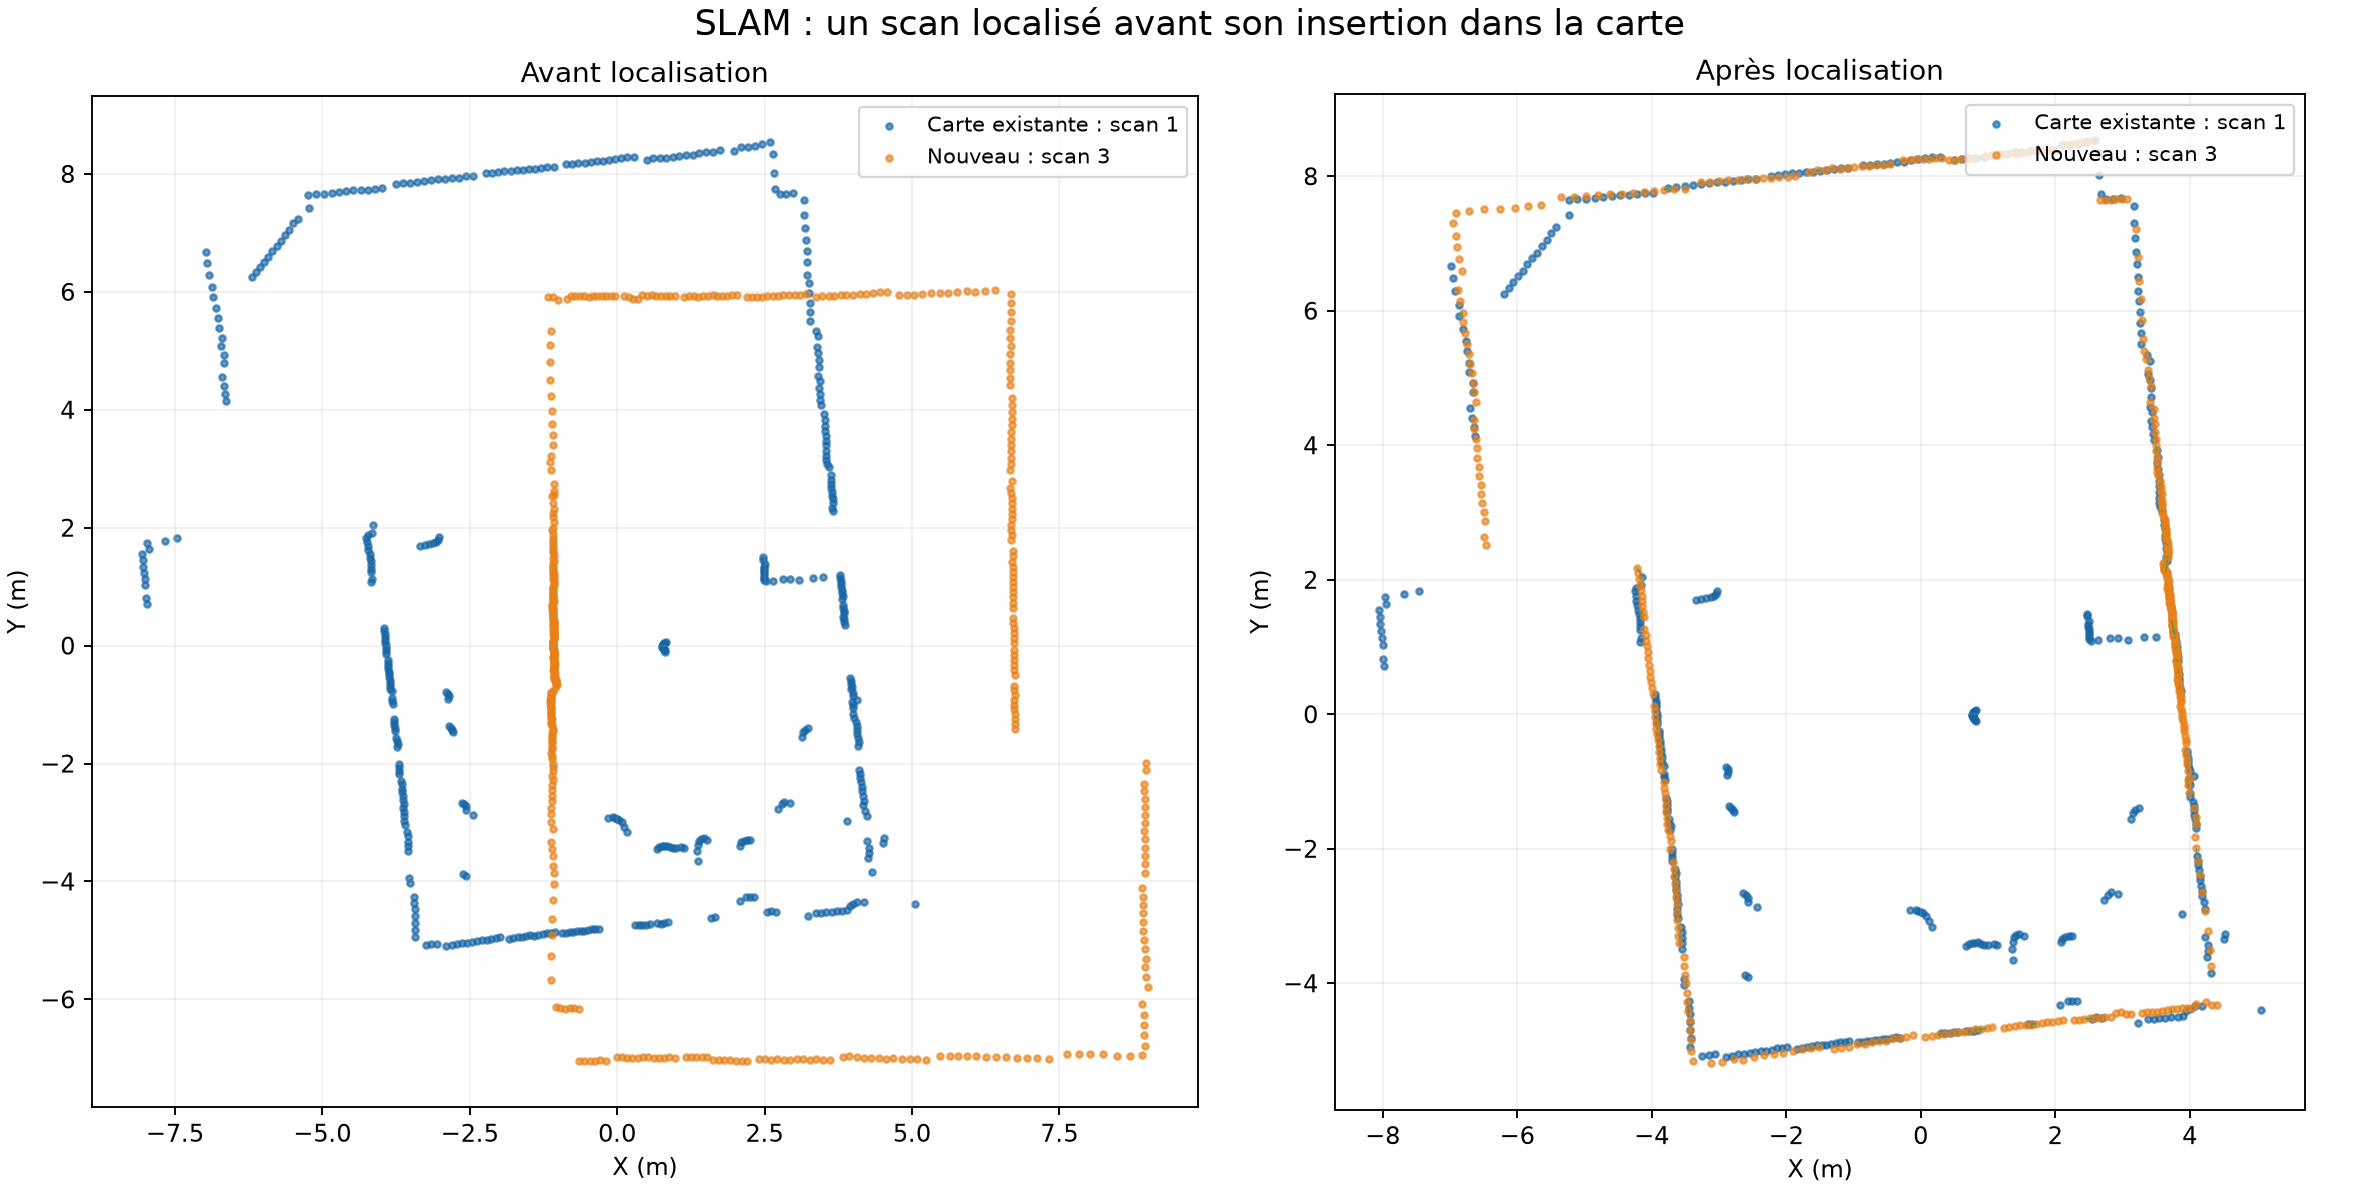
\includegraphics[width=.98\linewidth]{slam_recalage_scan3.png}
\caption{Localisation du scan 3 avant son insertion dans la carte. La pose
estimée est calculée depuis les scans, sans référence terrain mesurée.}
\end{figure}
La carte s'enrichit après chaque scan accepté. Les quatre panneaux montrent
le nuage global après 1, 3, 6 puis 9 scans, avec une couleur par acquisition.
\begin{figure}[H]\centering
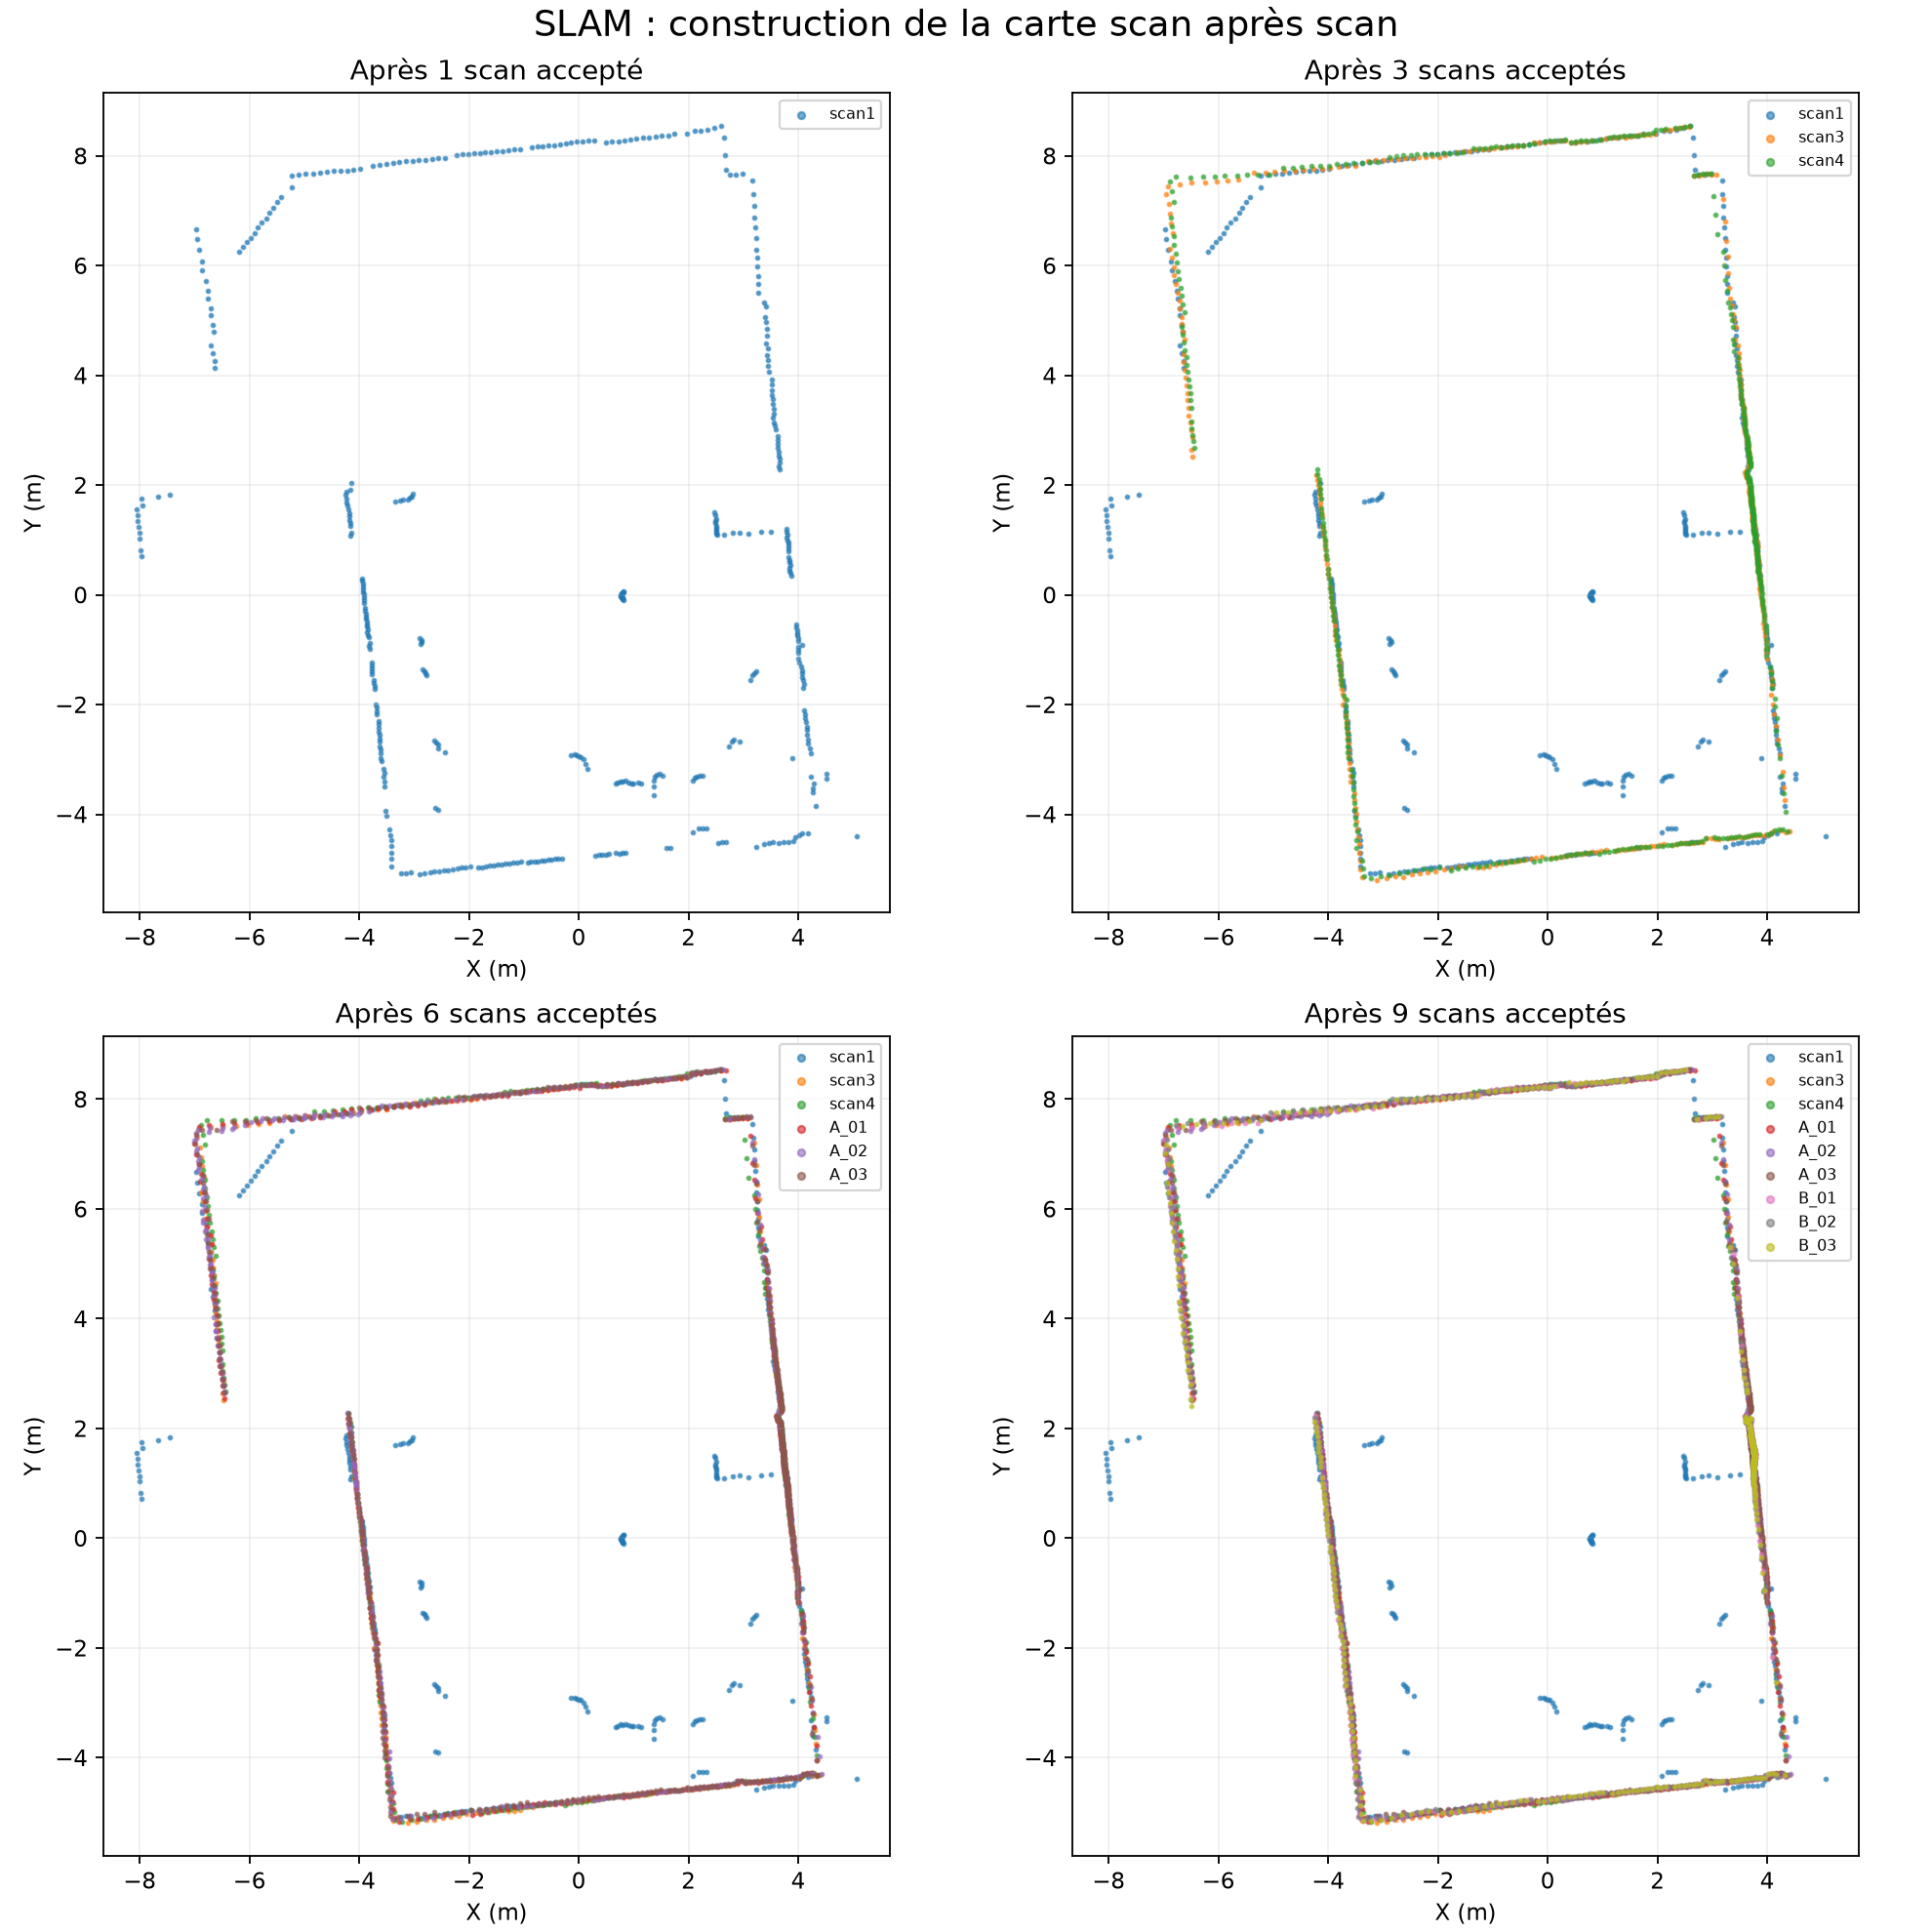
\includegraphics[width=.83\linewidth]{slam_progression_nuages.png}
\caption{Progression de la fusion incrémentale des points LiDAR. Le scan 2
n'apparaît pas dans la carte contrôlée parce que son score dépasse le seuil.}
\end{figure}

\section{Résultats calculés}
9 scans sur 10 ont été ajoutés, soit 4159 points
valides insérés. La carte vectorielle exportée contient 17 segments.
La grille allouée couvre X de -9.12 à 6.08 m et Y de -6.16 à
9.60 m ; ces bornes comprennent une marge de calcul et ne sont pas les
dimensions mesurées de la salle.

\begin{longtable}{lrrrrrrl}
\toprule Scan & Points & X (m) & Y (m) & $\theta$ ($^\circ$) & $<30$ cm & Score & Décision \\
\midrule\endhead
scan1 & 454 & 0.00 & 0.00 & 0.0 & -- & 0.000 & Ajouté \\
scan2 & 453 & -2.98 & 2.38 & 99.2 & 46\% & 0.189 & Écarté \\
scan3 & 456 & 2.65 & 1.45 & -174.2 & 87\% & 0.038 & Ajouté \\
scan4 & 457 & 2.62 & 1.47 & 95.3 & 100\% & 0.002 & Ajouté \\
A\_01 & 457 & 2.66 & 1.43 & -175.7 & 100\% & 0.001 & Ajouté \\
A\_02 & 519 & 2.66 & 1.45 & -175.7 & 100\% & 0.002 & Ajouté \\
A\_03 & 451 & 2.67 & 1.44 & -176.0 & 100\% & 0.002 & Ajouté \\
B\_01 & 456 & 3.55 & 1.54 & -176.7 & 100\% & 0.002 & Ajouté \\
B\_02 & 455 & 3.54 & 1.54 & -176.7 & 100\% & 0.002 & Ajouté \\
B\_03 & 454 & 3.54 & 1.55 & -176.5 & 100\% & 0.002 & Ajouté \\
\bottomrule
\end{longtable}
Les pourcentages comparent chaque scan au nuage cumulatif avant son insertion.
Le scan d'origine n'a pas de référence antérieure. Les scores ne sont pas des
erreurs de pose : les positions physiques n'ont pas été mesurées. Les temps et
scores détaillés sont dans \texttt{resultats/diagnostic.json} et
\texttt{resultats/poses\_et\_qualite.csv}. Le fichier scan2 a été écarté
par le contrôle de cohérence ; il reste conservé dans les données TP1.
Une seconde carte exploratoire ajoute ce scan pour montrer sa couverture
potentielle. Elle ne sert pas de résultat de référence, car son alignement
n'a pas passé le seuil de qualité choisi.

\begin{figure}[H]\centering
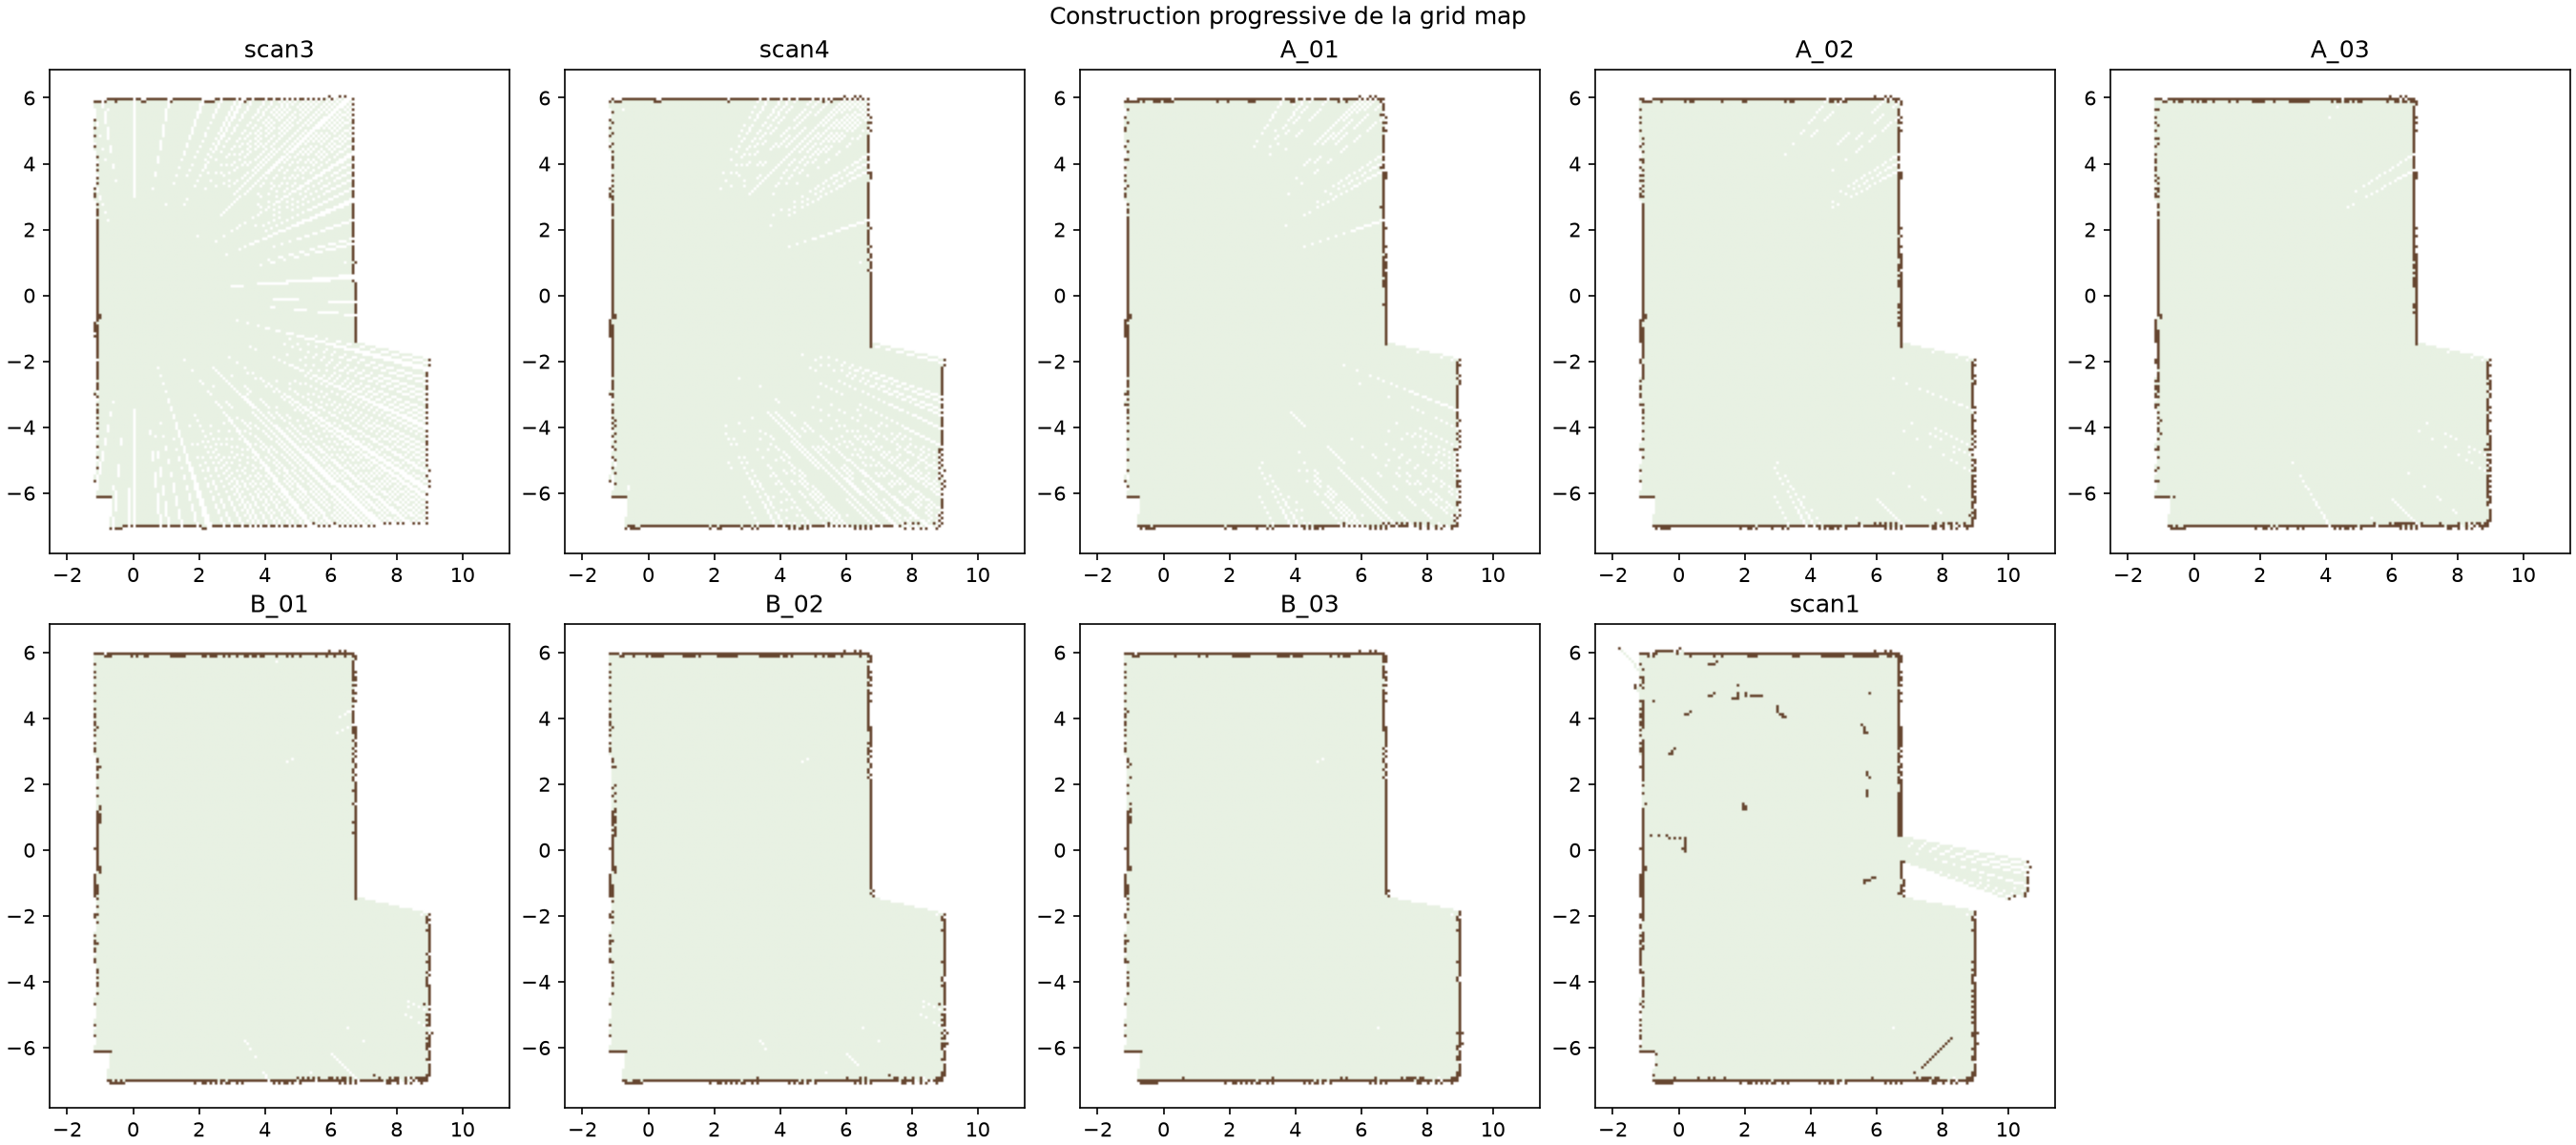
\includegraphics[width=.98\linewidth]{progression.png}
\caption{Construction progressive de la grid map. Chaque panneau montre la
carte après l'ajout d'un scan accepté. Blanc : inconnu ; vert : libre ; brun :
impact occupé.}
\end{figure}
\begin{figure}[H]\centering
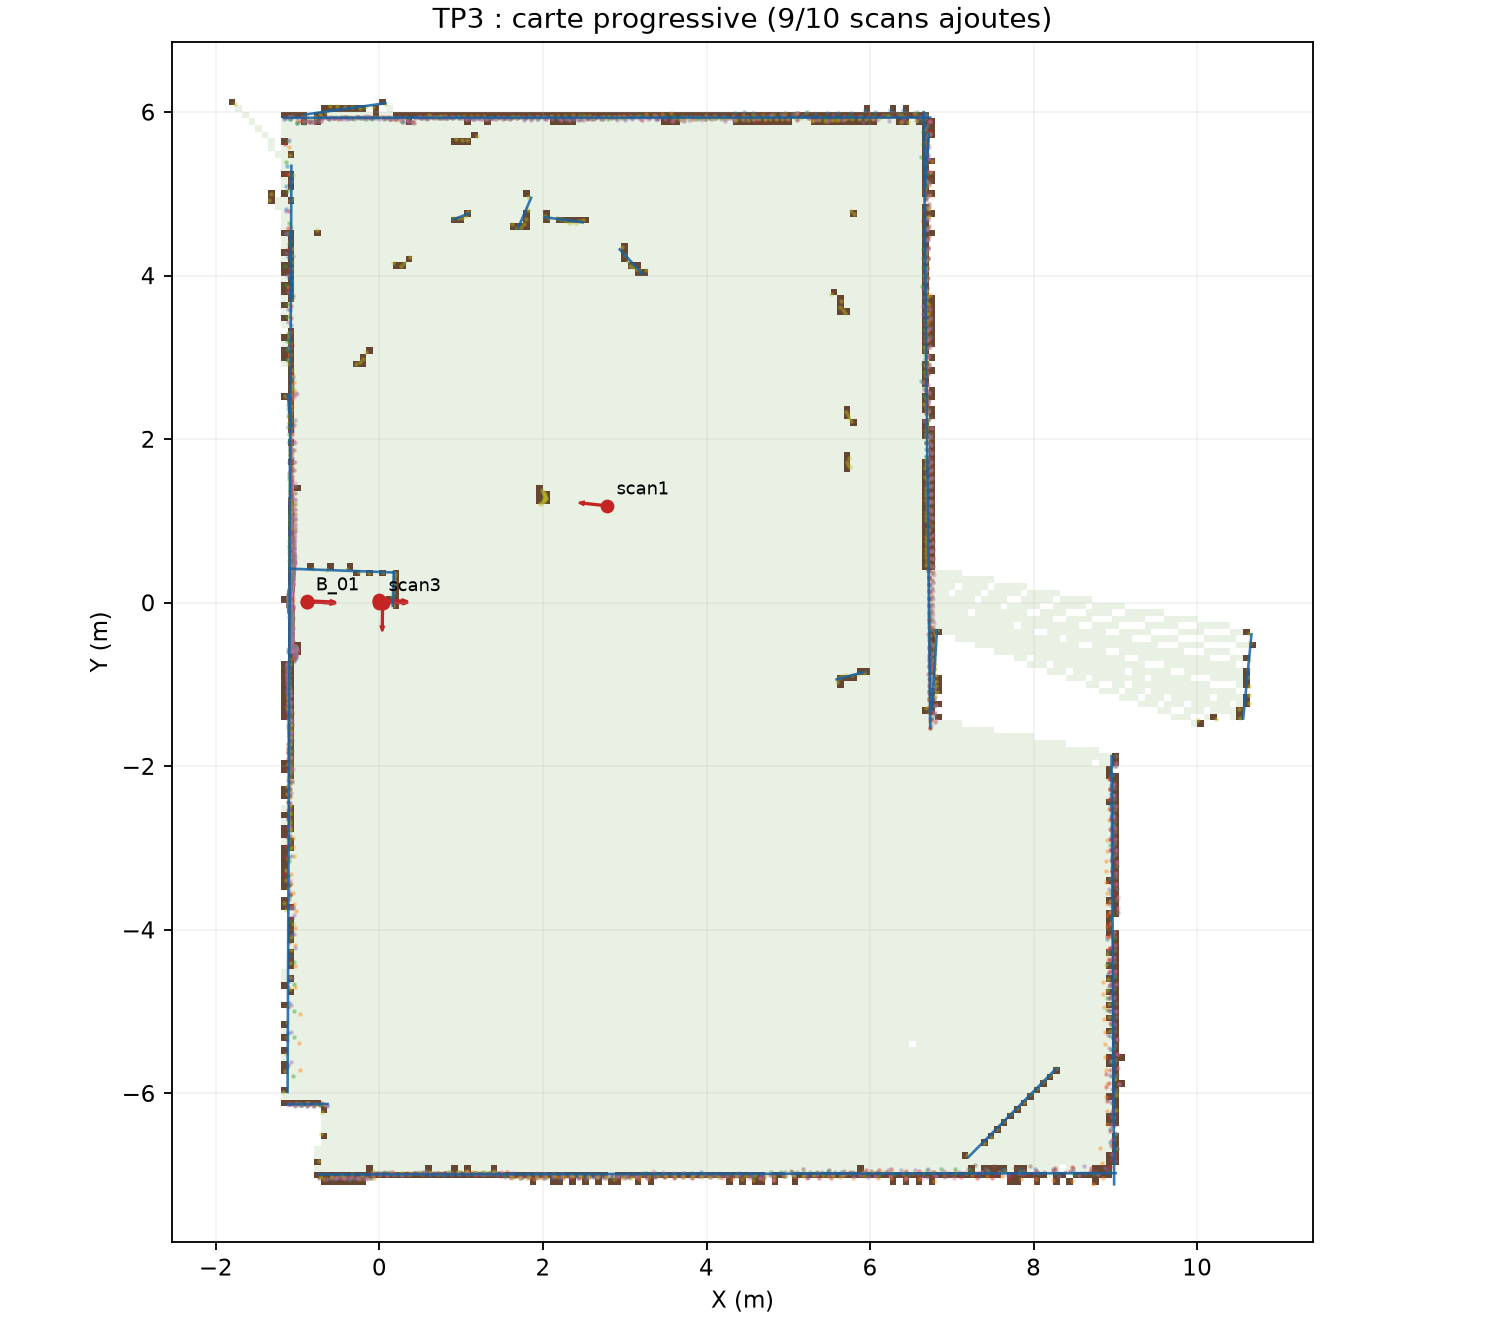
\includegraphics[width=.95\linewidth]{carte_finale.png}
\caption{Carte finale issue des scans acceptés. Les points colorés indiquent
les impacts ; les lignes bleues sont les segments vectoriels ; les marqueurs
rouges montrent les poses estimées.}
\end{figure}
\begin{figure}[H]\centering
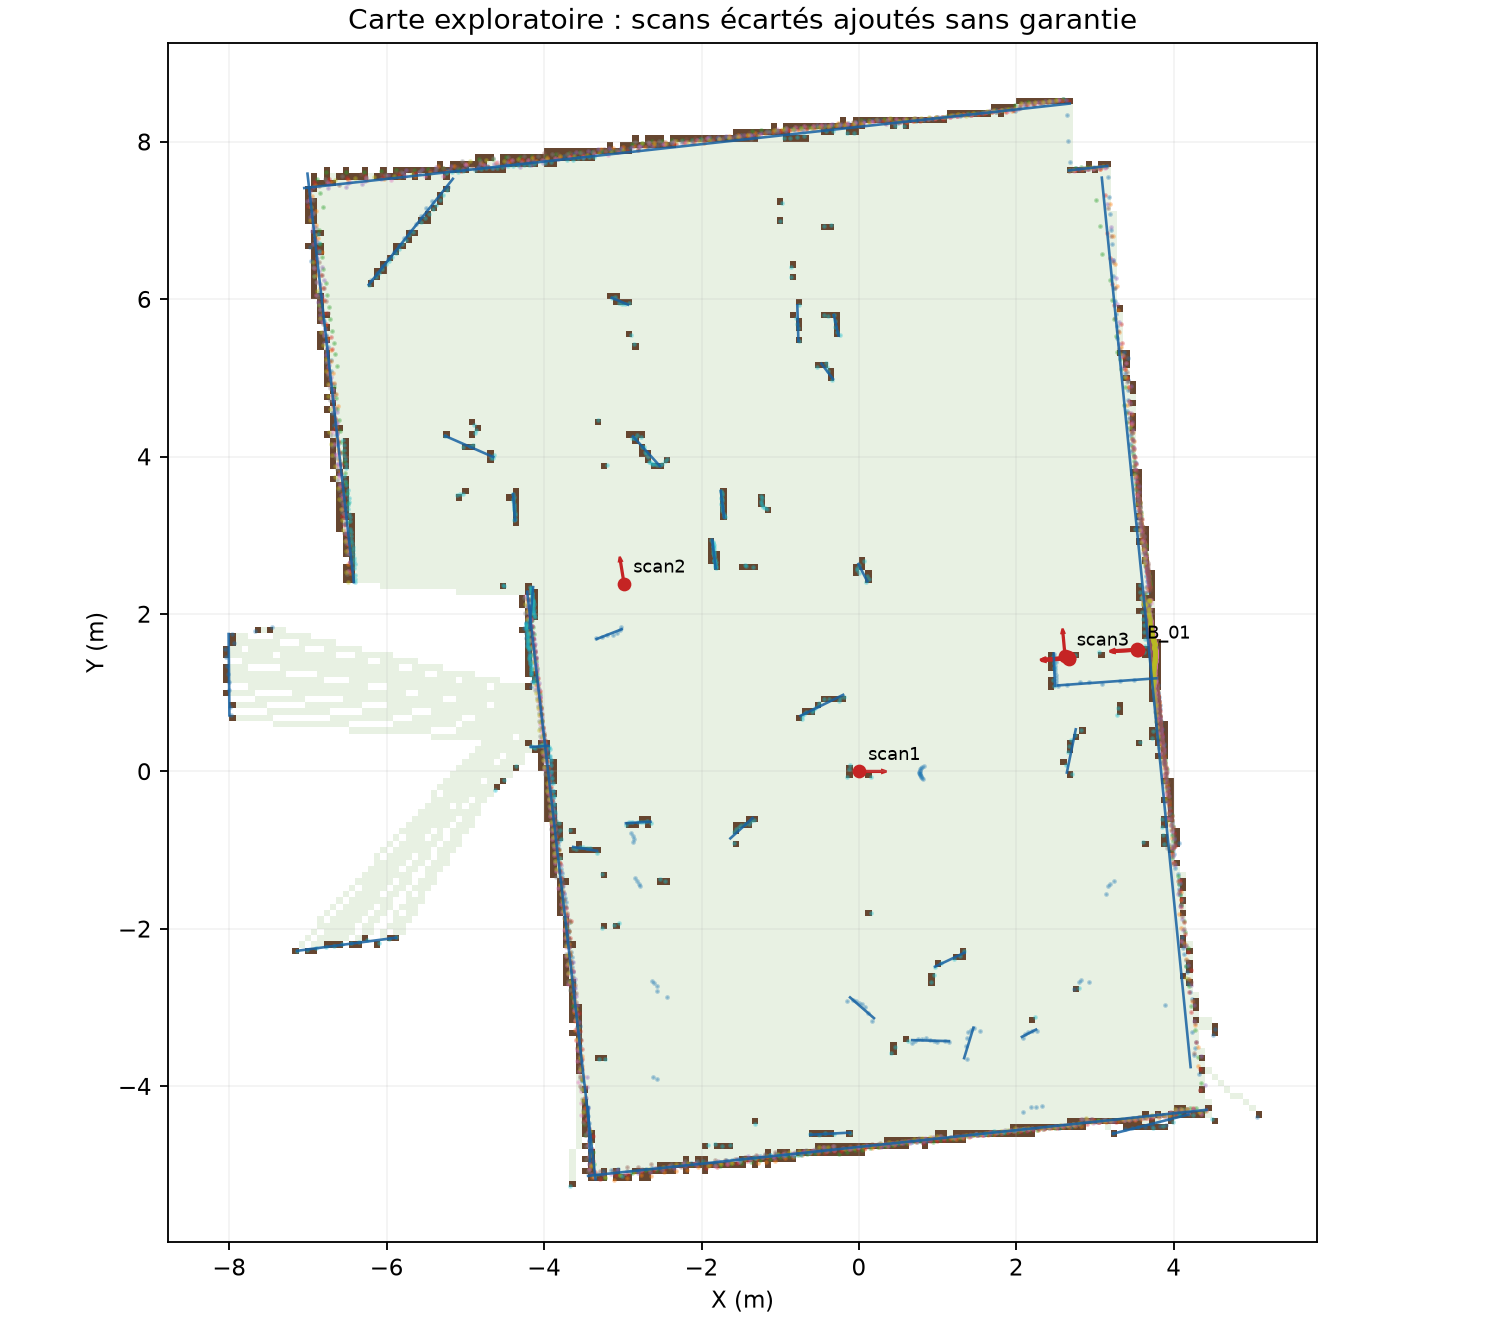
\includegraphics[width=.95\linewidth]{carte_exploratoire.png}
\caption{Carte exploratoire avec le scan écarté. La zone supplémentaire et ses
segments sont provisoires, faute de validation indépendante du recalage.}
\end{figure}

\section{Limites et suite du travail}
Les scans n'ont pas de poses terrain ni d'incertitudes de position et d'angle
mesurées indépendamment. On ne peut donc calculer ni erreur physique de la
carte ni taux de réussite réel. La répétition des tours A/B augmente la
densité des mesures, mais pas nécessairement la couverture spatiale. Les
parties blanches de la grille sont non observées et ne doivent pas être
interprétées comme libres. Une carte « complète » de toute la salle ne peut
pas être certifiée avec les seules données disponibles : il faut vérifier les
zones hors champ et refaire des acquisitions à hauteur constante là où des
surfaces restent cachées. Une fermeture de boucle, des références mesurées et
un relevé des murs permettraient une validation plus forte.


\section{Bonus : acquisitions avec le robot mobile}
Le robot ESP32 a fonctionné et a été déplacé par l'opérateur pendant la séance
d'acquisition. D'après les CSV fournis, 117 scans distincts ont été
enregistrés pendant cette séance. Le plus récent export cumulatif
comprend 114 scans ; quatre CSV individuels plus tardifs ont été ajoutés et un
doublon exact a été retiré. Les exports cumulatifs précédents contiennent les
mêmes premiers scans et ne sont donc pas additionnés. La hauteur du capteur et
les poses réelles du robot n'ont pas été relevées dans ces fichiers.

Le firmware suspend la lecture du LiDAR pendant une impulsion moteur. Un scan
renvoyé par le serveur pendant ce mouvement peut donc être ancien. Les commandes
de déplacement et les captures appartiennent à la même séance, mais les CSV ne
prouvent pas qu'un nouveau tour LiDAR ait été acquis pendant que les roues
tournaient. Le programme
bonus applique une boucle arrêt, scan frais, localisation ICP locale, mise à jour
de la grille, puis courte impulsion de mouvement. Il vérifie le dégagement frontal
et arrête le robot si le scan est absent, si le recalage échoue ou si un obstacle
est trop proche. Le pilotage automatique est disponible dans le code mais n'a
pas été exécuté sur le robot physique dans cette étude ; seul le rejeu des CSV
et les tests avec un faux robot ont été réalisés.

Le rejeu accepte 86 scans dans 13 sous-cartes.
Celles-ci possèdent des repères locaux indépendants : les pertes de localisation
interdisent de les superposer comme si leurs poses relatives étaient connues.
Les champs \texttt{pose\_x}, \texttt{pose\_y} et \texttt{pose\_angle\_deg} sont
renseignés manuellement par la route \texttt{/pose} du firmware ; ils ne sont pas
une vérité terrain et n'ont pas été employés pour le recalage.

Pour regrouper les sous-cartes dans un même dessin, la carte TP3 antérieure
sert de repère géométrique explicite. Une recherche grossière de translations
et rotations est affinée par ICP sur les cellules occupées. Sur les
13 sous-cartes, 6 raccords passent les seuils indicatifs de
35\% de cellules occupées à moins de 30 cm et de score inférieur ou égal à
0,12 m$^2$. Les autres restent incertains. Ces seuils n'ont pas été validés
par des poses terrain ; les couleurs et la superposition ne constituent pas
une carte globale métriquement certifiée. La grille de fond comprend des scans
antérieurs et ne mesure pas la seule couverture du robot mobile.


\begin{figure}[H]\centering
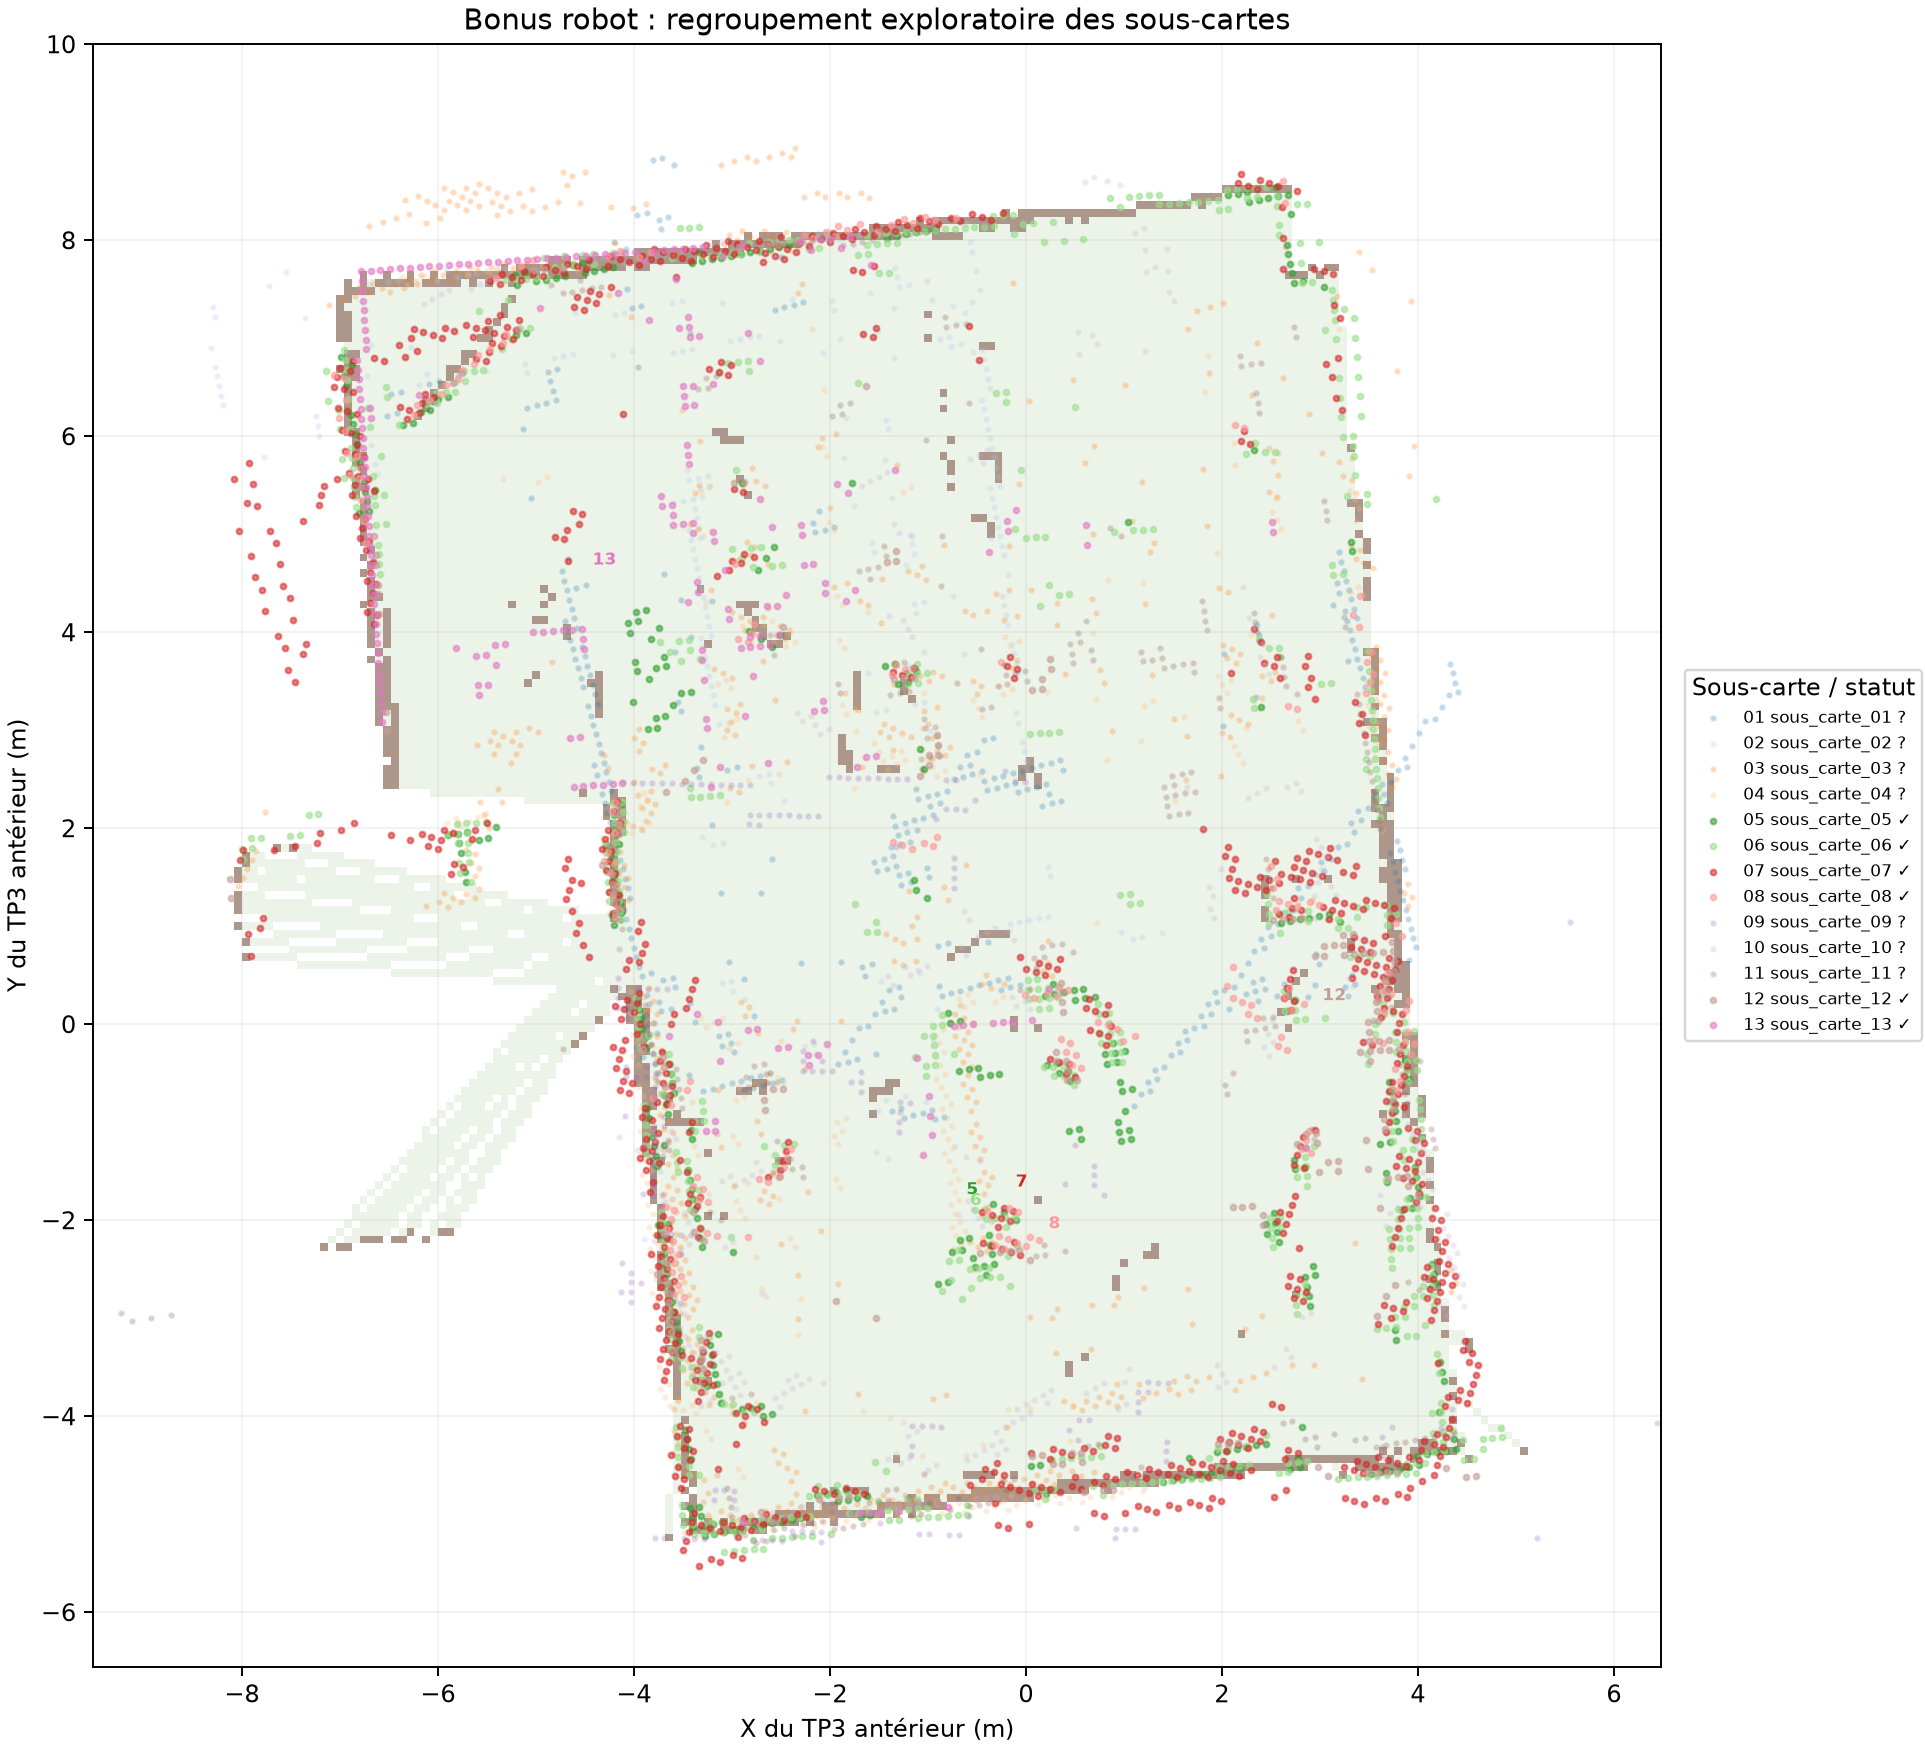
\includegraphics[width=.95\linewidth,height=.70\textheight,keepaspectratio]{../bonus_robot/resultats_rejeu/carte_regroupee_exploratoire.png}
\caption{Regroupement exploratoire des sous-cartes du robot sur la carte TP3
antérieure. Les couleurs vives indiquent les raccords plausibles selon le score
choisi ; les points pâles indiquent les raccords incertains.}
\end{figure}


\begin{longtable}{lrrrrrl}
\toprule Sous-carte & X (m) & Y (m) & $\theta$ ($^\circ$) & $<30$ cm & Score (m$^2$) & Statut \\
\midrule\endhead
sous\_carte\_01 & -0.95 & 1.56 & 15.3 & 48\% & 0.158 & Incertain \\
sous\_carte\_02 & -2.70 & 5.65 & -78.4 & 49\% & 0.159 & Incertain \\
sous\_carte\_03 & -1.83 & -1.07 & 152.7 & 47\% & 0.168 & Incertain \\
sous\_carte\_04 & -2.10 & -0.59 & -151.0 & 57\% & 0.137 & Incertain \\
sous\_carte\_05 & -0.61 & -1.74 & 10.3 & 64\% & 0.112 & Plausible \\
sous\_carte\_06 & -0.57 & -1.85 & 94.1 & 71\% & 0.092 & Plausible \\
sous\_carte\_07 & -0.10 & -1.66 & 72.8 & 73\% & 0.080 & Plausible \\
sous\_carte\_08 & 0.23 & -2.08 & -20.2 & 74\% & 0.082 & Plausible \\
sous\_carte\_09 & -3.35 & -1.30 & -1.3 & 54\% & 0.142 & Incertain \\
sous\_carte\_10 & -2.85 & -2.78 & 29.1 & 54\% & 0.137 & Incertain \\
sous\_carte\_11 & -0.44 & 2.86 & -80.3 & 59\% & 0.136 & Incertain \\
sous\_carte\_12 & 3.03 & 0.24 & -176.3 & 68\% & 0.098 & Plausible \\
sous\_carte\_13 & -4.42 & 4.69 & -176.0 & 62\% & 0.111 & Plausible \\
\bottomrule
\end{longtable}
Les poses du tableau sont des raccords estimés au repère du TP3 antérieur,
et non des déplacements mesurés du robot.

\begin{figure}[H]\centering
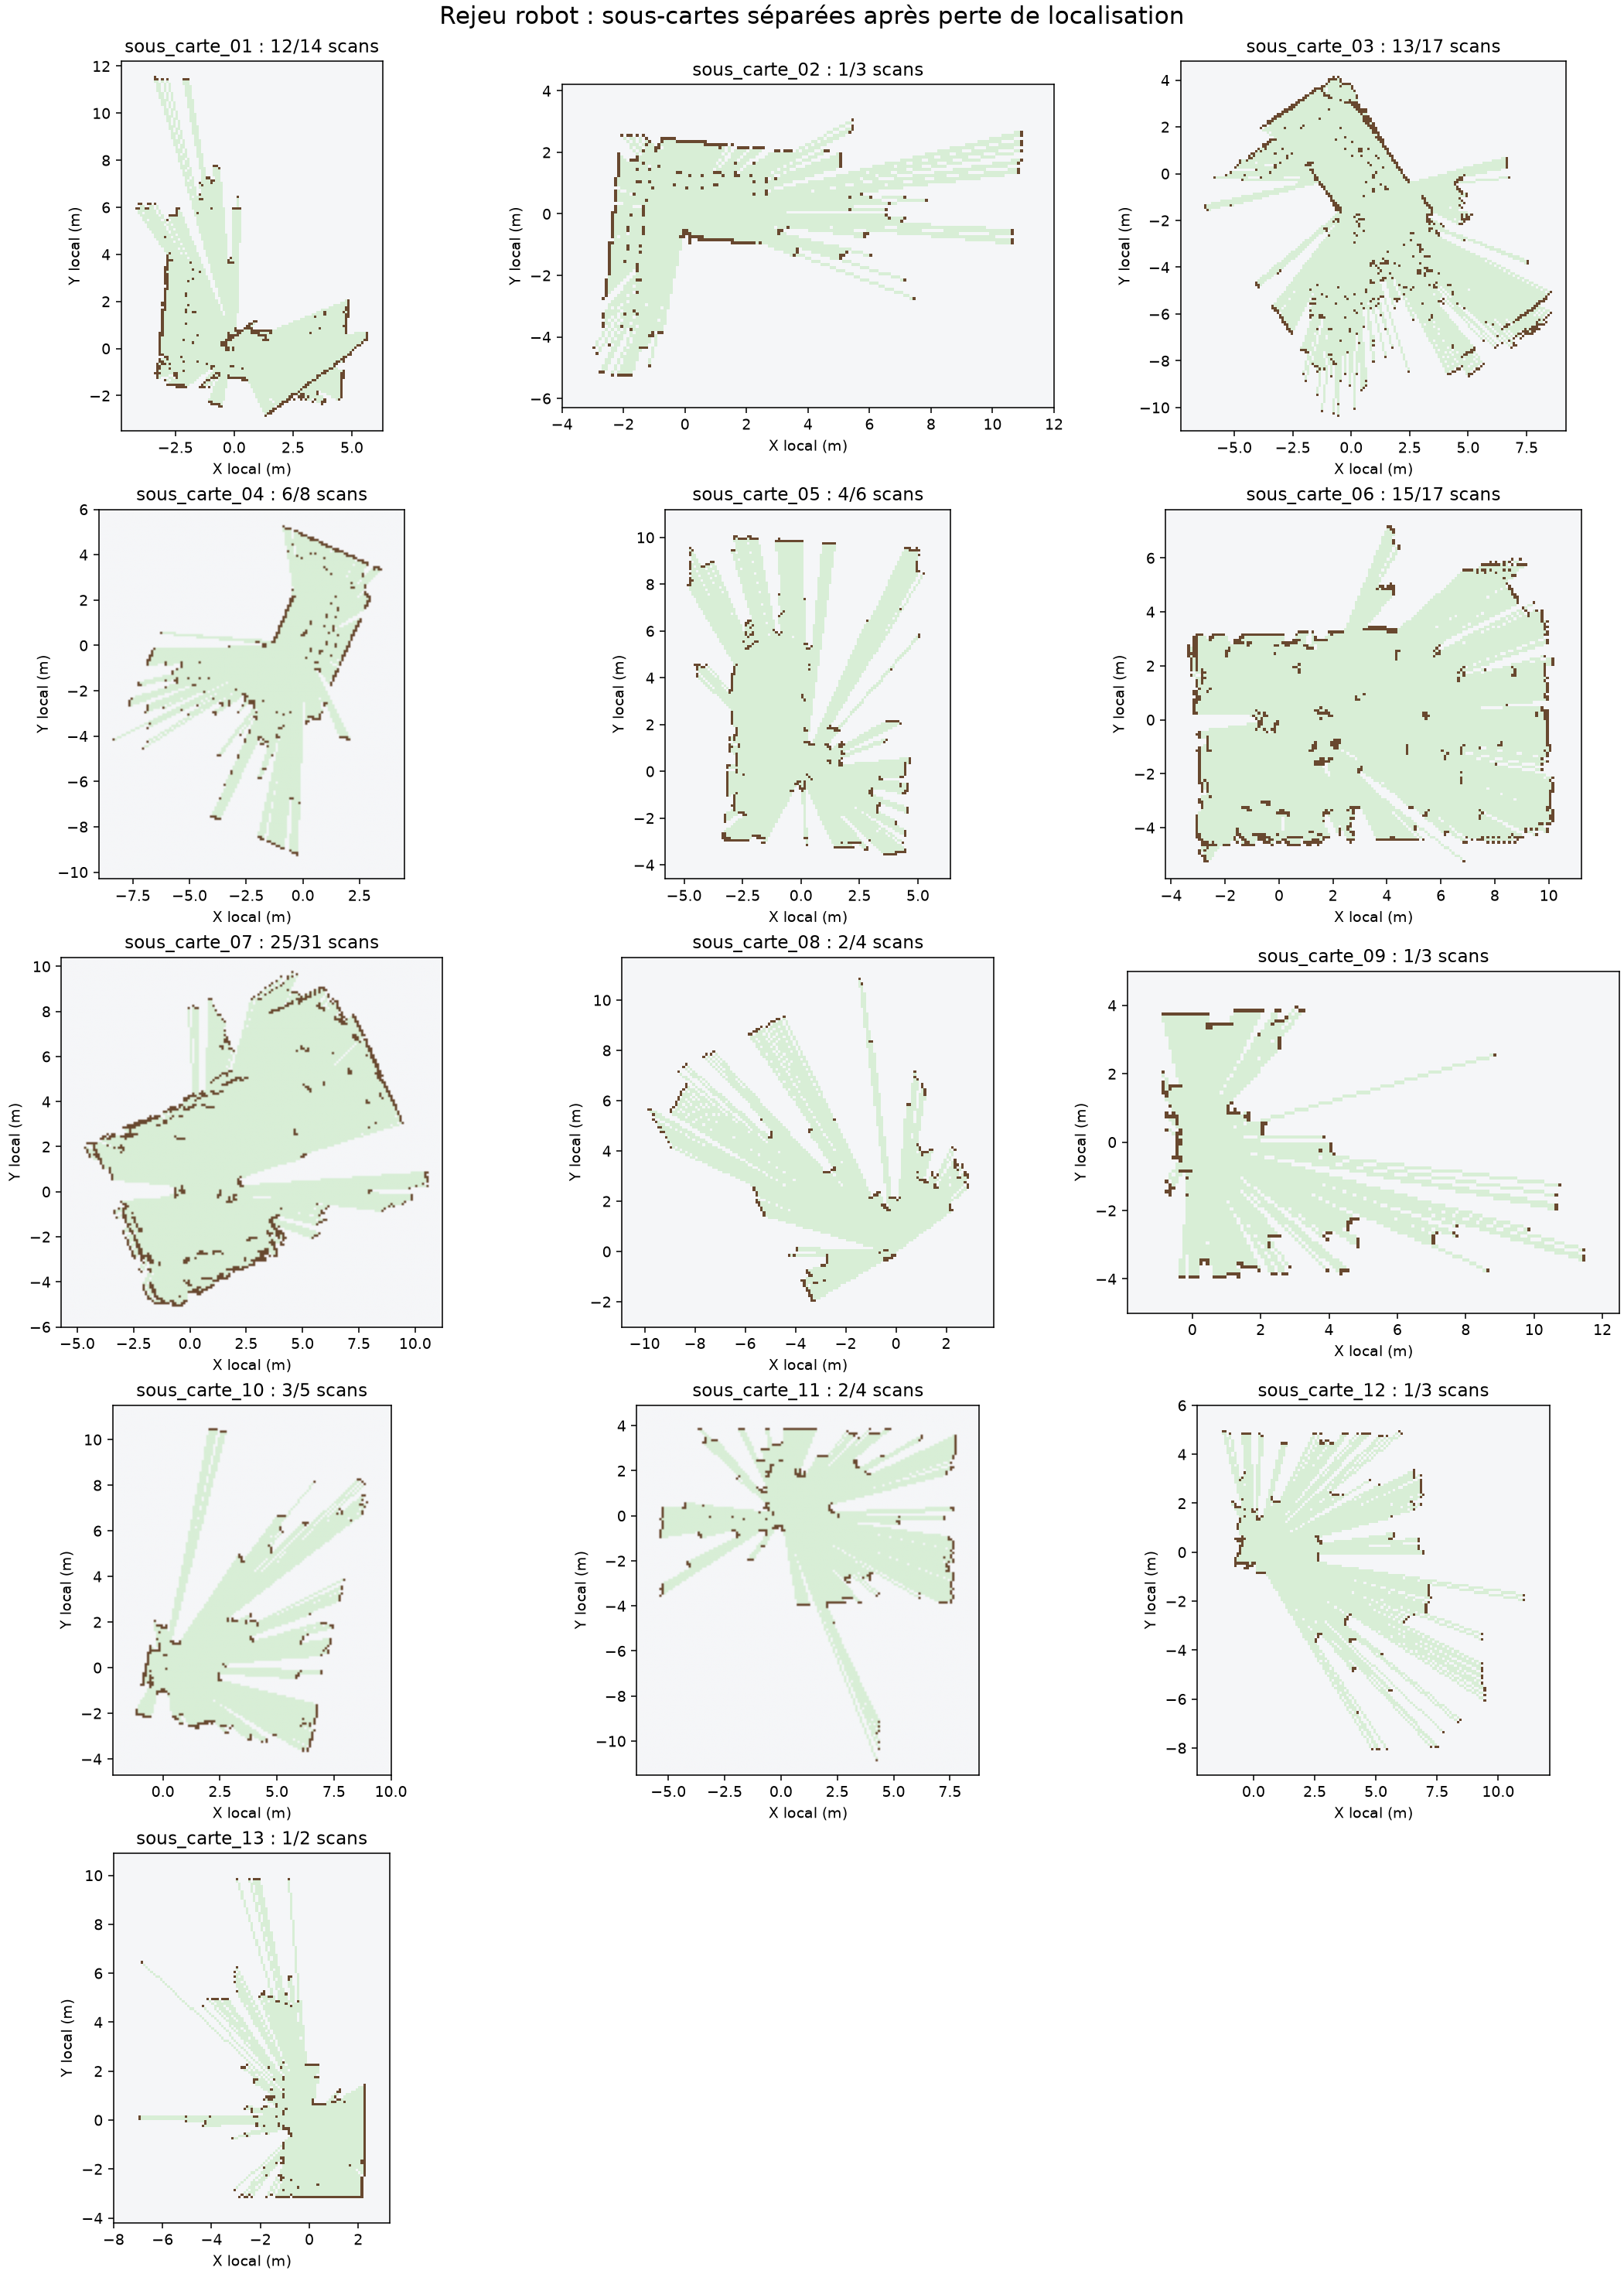
\includegraphics[width=.95\linewidth,height=.67\textheight,keepaspectratio]{../bonus_robot/resultats_rejeu/vue_sous_cartes.png}
\caption{Sous-cartes calculées à partir du déplacement du robot. Chaque panneau
possède son propre repère ; le blanc signifie non observé, le vert libre et le
brun occupé. Leur assemblage global reste à valider.}
\end{figure}
\begin{figure}[H]\centering
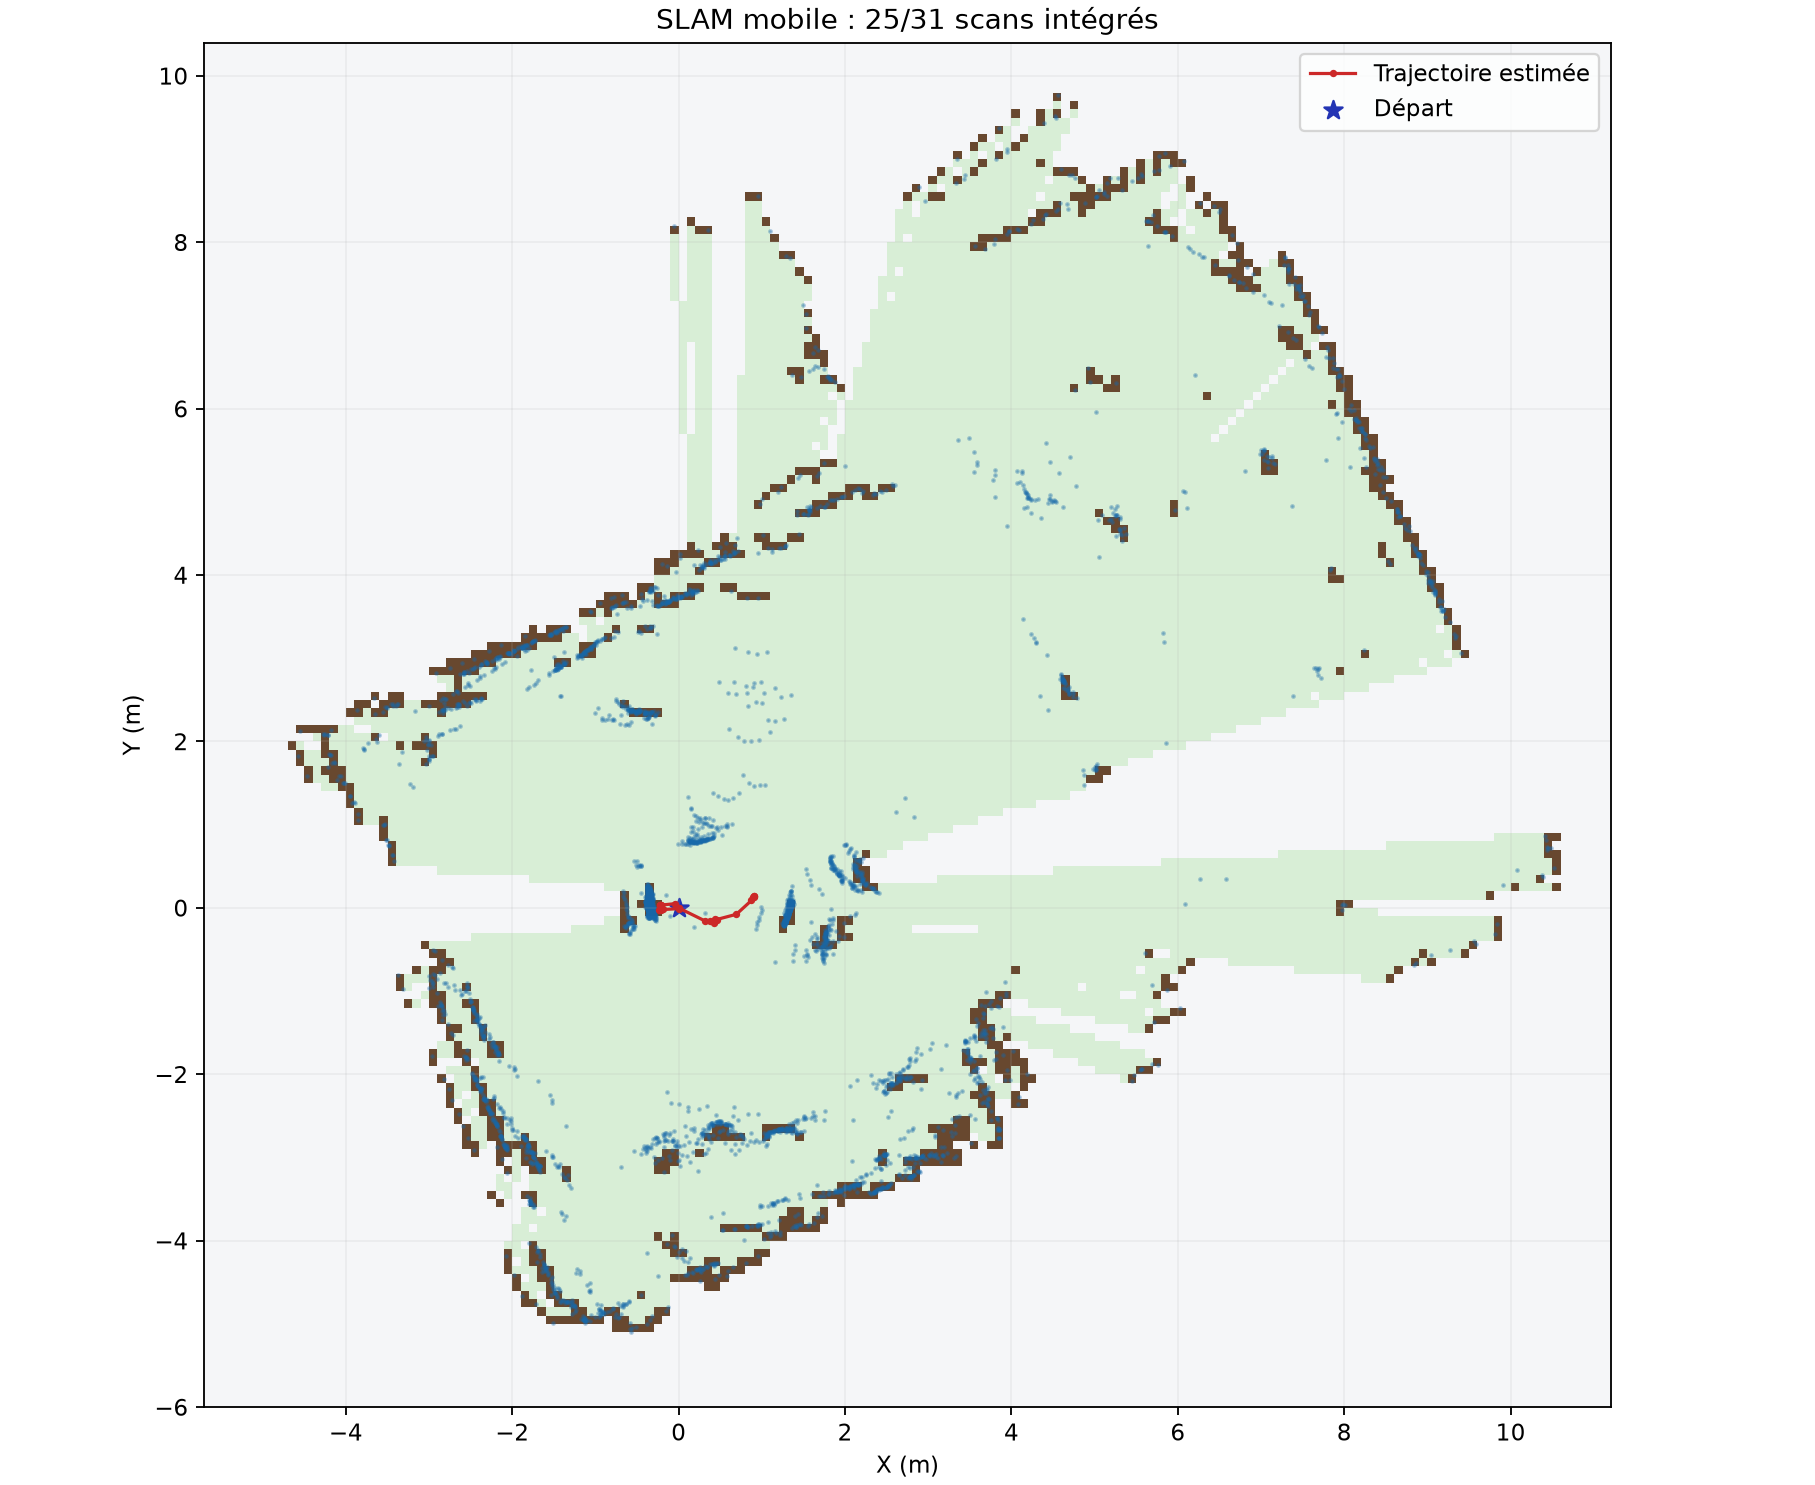
\includegraphics[width=.86\linewidth]{../bonus_robot/resultats_rejeu/sous_carte_07/slam_mobile.png}
\caption{Séquence locale la plus longue : grille et trajectoire estimée dans
la sous-carte 07. Aucune erreur absolue ne peut être calculée sans mesures de
position indépendantes.}
\end{figure}

\section{Reproduction}
Depuis la racine du dépôt :
\begin{verbatim}
python -m pip install -r tp1/LD06_Atelier/requirements.txt
python tp3/slam.py
python tp3/generer_figures_slam.py
python tp3/creer_rapport.py
python -m unittest discover -s tp3 -p "test_*.py" -v
\end{verbatim}
Compiler ensuite \texttt{tp3/rapport/rapport\_tp3.tex} depuis son dossier.
Les CSV, JSON, figures et cartes exportées sont dans \texttt{tp3/resultats/}.
\end{document}
